\begin{egBox}{Separation Axioms}[eg:31.1]
    It is clear that a regular space is Hausdorff, and that a normal space is
    regular.
    Notice that we needed to include the condition that one-point sets be
    closed as a part of the definition of regularity and normality in order 
    for this to be the case; a two-point space in the trivial topology satisfies
    the other part of the definitions of regularity and normality, even though
    it is not Hausdorff.

    \baseSkip

    Hausdorff, regular, and normal are all called \textbf{separation axioms}
    for the reason that they involve "separating" certain kinds of sets from
    one another by disjoint open sets.
    We have used the word "separation" before, of course, when we studied
    connected space. But in that case, we were trying to find disjoint open sets
    whose \textit{union was the entire space}.
    The present situation is quite different because the open sets need not
    satisfy this condition.

    \baseSkip

    \begin{figure}[H]
        \centering
        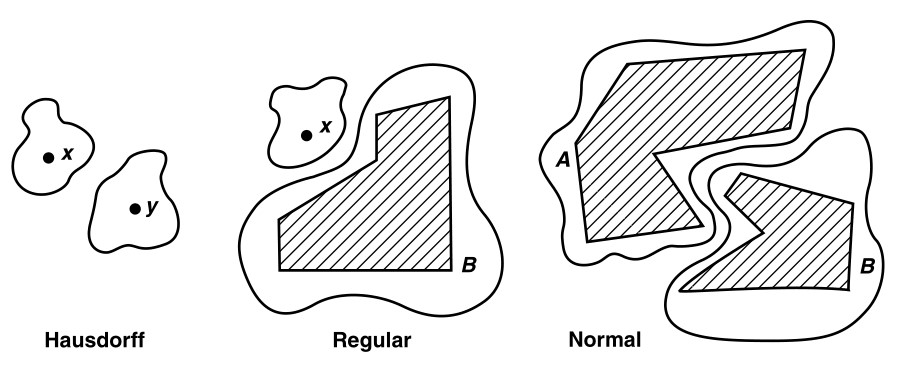
\includegraphics[ width = 0.6\linewidth ]{figures/Section 31/eg31-1.jpg}
        \caption{The three separation axioms illustrated}
        \label{fig:31-1}
    \end{figure}
\end{egBox}

\begin{egBox}{Regular but not Hausdorff}[eg:31.2]
    Let \( \mathbb{R}_{ K } \) be \( \mathbb{R} \) with the \( K \)-topology,
    which is the topology that is almost the standard topology, except 
    \( K \) is deemed \textit{closed}.

    \baseSkip

    \( K \) is closed in \( \mathbb{R}_{ K } \) and \( 0 \notin K \).
    Notice that there exists open neighborhoods of \( 0 \) that does not
    intersect with \( K \) -- e.g., \( \mathbb{R} \setminus K \).
    However, \( 0 \) and \( K \) can't be separated by disjoint open 
    neighborhoods. 
    Thus, we have that \( \mathbb{R}_{ K } \) is not regular.
    On HW, we have already shown that \( \mathbb{R}_{ K } \) is Hausdorff.
\end{egBox}